\documentclass{article}

\usepackage{amsmath, mathtools, amsthm}

\usepackage{graphicx}
\graphicspath{ {./images/} }

\title{Onde elettromagnetiche}
\author{github.com/asdrubalini}
\date{\today}

\begin{document}
    \maketitle

    \section{Onda elettromagnetica}

    Come suggerisce il nome, un'onda elettro-magnetica è una combinazione di un'onda elettrica ed un'onda
    magnetica che si propaga all'interno dello spazio e che è in grado di trasportare energia da un punto di
    partenza ad un punto di arrivo.
    
    \section{Definizione del campo elettrico}

    Il campo elettrico si rappresenta con la lettera E e viene definito come:

    \begin{equation}
        \bar{E}^+(x, t) = E^+_M \cdot e^{j\omega (t-\frac{x}{u})}
    \end{equation}

    Con $k$ si indica la costante di fase che è definita con seguente rapporto

    \begin{equation}
        k = \frac{\omega}{u}
    \end{equation}

    quindi

    \begin{equation}
        \bar{E}^+(x, t) = E^+_M \cdot e^{j (\omega t - kx)}
    \end{equation}

    \section{Definizione del campo magnetico}

    Il campo magnetico si rappresenta con la lettera H e viene definito come:

    \begin{equation}
        \bar{H}^+(x,t) = \frac{\bar{E}^+(x,t)}{Z}
    \end{equation}

    dove $Z$ è l'impedenza caratteristica misurata in ohm $[\Omega]$

    \section{Velocità di onde elettromagnetiche}

    La velocità di un'onda elettromagnetica è costante e si può calcolare con

    \begin{equation}
        u = \frac{1}{\sqrt{\varepsilon \mu}} \hspace{0.2cm} [m/s]
    \end{equation}

    dove $\mu$ è la permeabilità magnetica e $\varepsilon$ è la permittività elettrica.
    Nel vuoto, la formula diventa

    \begin{equation}
        c = \frac{1}{\sqrt{\varepsilon_0 \mu_0}} = 299 792 458 \hspace{0.2cm} [m/s]
    \end{equation}

    \vspace{1cm}

    La permeabilità magnetica si può esprimere come il prodotto

    \begin{equation}
        \mu = \mu_0 \mu_r
    \end{equation}

    dove $\mu_0$ è la permeabilità magnetica del vuoto e $\mu_r$ è la permeabilità magnetica relativa
    del materiale.

    \vspace{1cm}

    Allo stesso modo, la permittività elettrica si può esprimere come il prodotto

    \begin{equation}
        \varepsilon = \varepsilon_0 \varepsilon_r
    \end{equation}

    dove $\varepsilon_0$ è la permittività elettrica del vuoto e $\varepsilon_r$ è la permittività elettrica relativa
    del materiale.

    \section{Impedenza caratteristica}

    L'impedenza caratteristica del vuoto è costante e si può calcolare con

    \begin{equation}
        Z_0 = \sqrt{\frac{\mu_0}{\varepsilon_0}} = c_0 \mu_0 \approx 377 \hspace{0.2cm} [\Omega]
    \end{equation}

    In generale, l'impedenza caratteristica di un mezzo diverso dal vuoto si calcola con

    \begin{equation}
        Z = \sqrt{\frac{\mu}{\varepsilon}} = c \mu = Z_0 \frac{u}{c} \hspace{0.2cm} [\Omega]
    \end{equation}

    \begin{equation}
        Z = Z_0 \sqrt{\frac{\mu_r}{\varepsilon_r}} \hspace{0.2cm} [\Omega]
    \end{equation}

    \section{Lunghezza d'onda, frequenza e altre caratteristiche di un'onda}

    Con la lettera greca lambda si rappresenta la lunghezza d'onda che si misura in metri.

    \begin{equation}
        \lambda = u T = \frac{u}{f} \hspace{0.2cm} [m]
    \end{equation}

    \begin{equation}
        \lambda = \frac{\omega}{k f}
    \end{equation}

    Da cui ricaviamo che la costante di fase (k) si può calcolare, sapendo la lunghezza d'onda, con:

    \begin{equation}
        k = \frac{2 \pi}{\lambda}
    \end{equation}

    \section{Riflessione di un'onda}

    \subsection{Coefficiente di riflessione}

    Quando un'onda elettro-magnetica passa da un dielettrico ad un altro, una parte dell'onda procede per la sua strada
    trapassando il dielettrico, mentre un'altra parte viene riflessa indietro con un angolo variabile.

    Il coefficiente di riflessione, misurato con la lettera K, indica la percentuale dell'onda che viene riflessa, in relazione
    a quella che invece trapassa il dielettrico.

    Se con $E^+_1$ indichiamo l'onda originale prima di trapassare il dielettrico e con $E^-_1$ indichiamo l'onda riflessa,
    è possibile calcolare il coefficiente di riflessione con:

    \begin{equation}
        K = \frac{E^-_1(x,t)}{E^+_1(x,t)}
    \end{equation}

    Nel caso in cui $K = 1$, possiamo dire che l'onda viene riflessa completamente. Inversamente, se $K = 0$, l'onda non viene
    riflessa neanche in minima parte.

    \subsection{Indice di rifrazione}

    Con rifrazione si intende la parte di onda elettro-magnetica che non viene riflessa ma riesce ad incidere il materiale
    passando dall'altra parte. L'angolo dell'onda rifratta rispetto alla normale varia in base alle caratteristiche dei due
    materiali. Ogni materiale ha un indice di rifrazione caratteristico indicato con la lettera $n$ e definito come:

    \begin{equation}
        n = \frac{c}{u}
    \end{equation}

    dove $c$ è la velocità della luce e $u$ è la velocità di propagazione nel materiale. L'indice di rifrazione è un valore $n = 1$
    per il vuoto ed $n < 1$ per tutti gli altri materiali. L'indice di rifrazione, inoltre, non ha unità di misura.

    \subsection{Angolo di riflessione}

    \begin{center}
        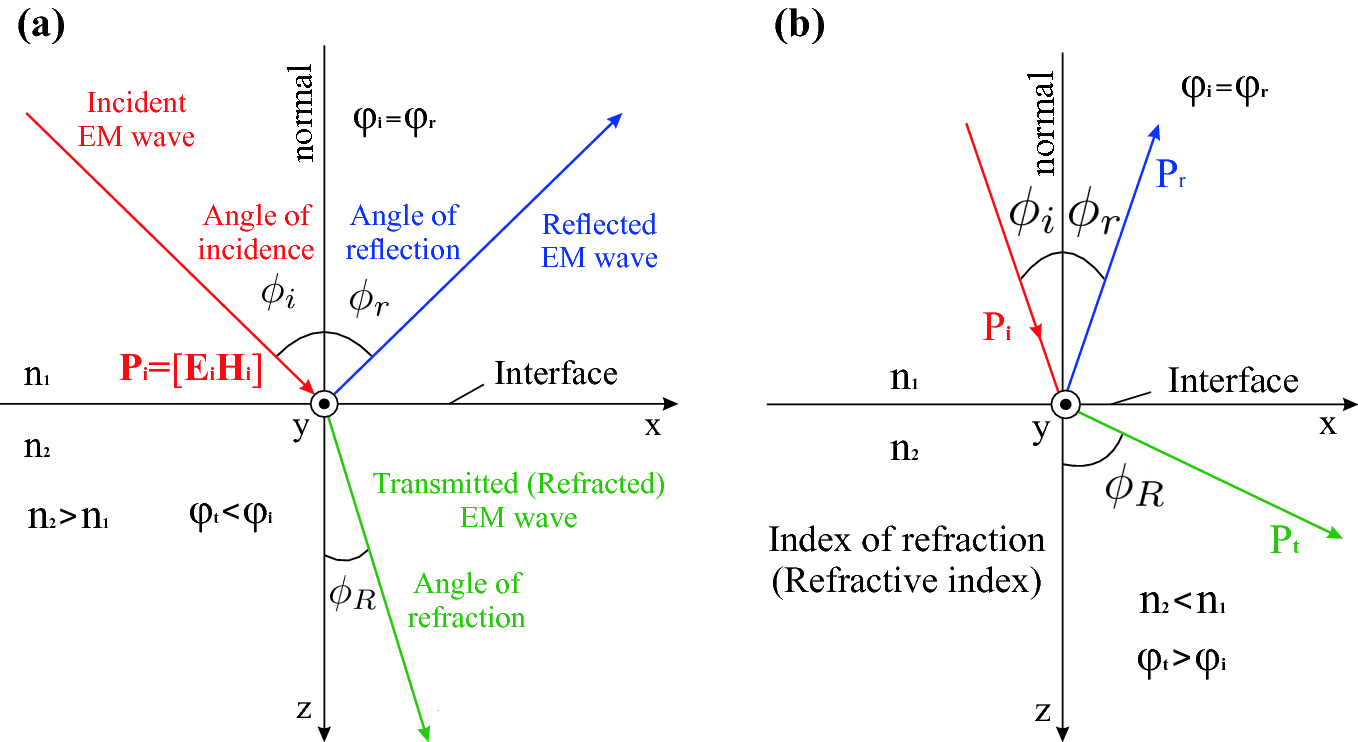
\includegraphics[width=\textwidth]{angolo-di-riflessione.png}
    \end{center}

    La legge di Snell definisce il seguente rapporto tra angolo di incidenza, rifrazione e indici di rifrazione dei mezzi:

    \begin{equation}
        \frac{sin(\phi_i)}{sin(\phi_R)} = \frac{n_2}{n_1}
    \end{equation}

    Se indichiamo con $\phi_i$ l'angolo con cui l'onda indice la superficie di separazione, con $\phi_r$ l'angolo con cui l'onda
    viene riflessa e con $\phi_R$ l'angolo con cui l'onda viene rifratta, le seguenti uguaglianze sono verificate:

    \begin{equation}
        \phi_i = \phi_r
    \end{equation}

    \begin{equation}
        \phi_R = arcsin(\frac{n_1 sin(\phi_i)}{n_2})
    \end{equation}

    \subsection{Angolo limite}

    Aumentando l'angolo di incidenza, aumenta conseguentemente anche l'angolo dell'onda rifratta. L'angolo di incidenza che consente
    all'onda rifratta di raggiungere i 90 gradi si definisce angolo limite. Applicando la legge di Snell, è possibile calcolare
    l'angolo limite con:

    \begin{equation}
        \phi_L = arcsin(\frac{n_2}{n_1})
    \end{equation}

    una volta raggiunto l'angolo limite, avremo un caso di riflessione totale, ovvero l'onda non viene rifratta ma soltanto riflessa.
    Si tratta dello stesso principio utilizzato dalla fibra ottica per trasmettere la luce a grandi distanze.

    \section{Densità di potenza}
    
    Il campo elettromagnetico, essendo composto da una part di campo elettrico (E) ed una parte di campo magnetico
    (H), ha associata una potenza S che rappresenta l'energia che nell'unità di tempo attraversa una sueprficie.

    \begin{equation}
        S = \frac{1}{2} E_M H_M
    \end{equation}

    Dove $H_M = \frac{E_M}{\zeta}$, quindi:

    \begin{equation}
        S = \frac{1}{2} \frac{{E_M}^2}{\zeta} \hspace{0.2cm} [\frac{W}{m^2}]
    \end{equation}

    \newpage

    \section{Linee di trasmissione}

    Una linea di trasmissione non è altro che una linea realizzata con due fili conduttori. Ogni linea può essere descritta
    con 4 costanti, chiamate costanti primarie. 

    \begin{itemize}
        \item R: tiene conto della resistenza
        \item L: tiene conto dei campi magnetici
        \item G: tiene conto delle perdite
        \item C: tiene conto dei campi elettrici
    \end{itemize}

    \subsection{Impedenza caratteristica}

    Con $\bar{Z_0}$ si definisce l'impedenza caratteristica della linea, calcolabile con la seguente formula:

    \begin{equation}
        \bar{Z_0} = \frac{\sqrt{R + j \omega L}}{\sqrt{G + j \omega C}} \hspace{0.2cm} [\Omega]
    \end{equation}

    \subsection{Costante di propagazione}

    \begin{equation}
        \bar{\varphi} = \sqrt{(R + j \omega L)(G + j \omega C)}
    \end{equation}

    Che può anche essere definita come la somma complessa di:

    \begin{equation}
        \bar{\varphi} = \alpha + j \beta
    \end{equation}

    dove $\alpha$ è la costante di attenuazione (che indica l'attenuazione del segnale) e $\beta$ è la 
    costante di fase (che indica lo sfasamento del segnale).

    \subsection{Coefficiente di riflessione}

    La linea si trova in regime stazionario quando ci sono sia onde progressive che onde regressive.
    Si definisce $\bar{K_L}$ il coefficiente di riflessione sul carico, che indica in che percentuale l'onda viene
    riflessa.

    \begin{equation}
        \bar{K_L} = \frac{
            \bar{Z_L} - \bar{Z_0}
        }{
            \bar{Z_L} + \bar{Z_0}
        }
    \end{equation}

    dove $\bar{Z_L}$ è l'impedenza sul carico.

    \subsection{Indice di riflessione relativo alla distanza dal carico}

    \begin{equation}
    \bar{K}(d) = \bar{K}_L \cdot e^{-j \beta d}
    \end{equation}

    dove $\beta$ si calcola con

    \begin{equation}
        \beta = \frac{2 \pi}{\lambda}
    \end{equation}

    \subsection{Impedenza relativa alla distanza dal carico}

    L'impedenza varia in base alla distanza a cui ci troviamo dal carico. Per calcolare l'impedenza ad una distanza nota,
    si usa la seguente formula:

    \begin{equation}
        \bar{Z}(d) = \bar{Z_0} \frac{
            \bar{Z_L} + j \bar{Z_0} tan(\beta d)
        }{
            \bar{Z_0} + j \bar{Z_L} tan(\beta d)
        }
    \end{equation}

    oppure

    \begin{equation}
        \bar{Z}(d) = \bar{Z}_0 \frac{
            1 + \bar{K}(d)
        }{
            1 - \bar{K}(d)
        }
    \end{equation}



    \subsection{Rapporto onda stazionaria}

    Il ROS è una misura del disadattamento di impedenza tra la linea di trasmissione ed il suo carico. Il suo valore minimo
    è 1 e corrisponde alla condizione di perfetto adattamento. I valori maggiori indicano un disadattamento dovuti ad una
    riflessione parziale del carico.

    \begin{equation}
        ROS = \frac{Vmax}{Vmin} =
        \frac{Imax}{Imin} =
        \frac{
            1 + |\bar{K_L}|
        }{
            1 - |\bar{K_L}|
        }
    \end{equation}

    \subsection{Linea ideale}

    Una linea ideale è una linea con perdite nulle, in cui si verificano le seguenti condizioni:

    \begin{equation}
        \alpha = 0
    \end{equation}

    \begin{equation}    
        \beta = \omega \sqrt{LC}
    \end{equation}

    \subsection{Linea adattata}

    Una linea adattata è una linea senza riflessioni, paragonabile ad una linea di lunghezza infinita.
    Nelle linee adattate si verifica che l'impedenza del carico è uguale all'impedenza caratteristica.

    \begin{equation}
        \bar{Z_L} = \bar{Z_0}
    \end{equation}

    Pertanto, il coefficiente di riflessione è zero:

    \begin{equation}
        \bar{K_L} = \frac{
            \bar{Z_L} - \bar{Z_0}
        }{
            \bar{Z_L} + \bar{Z_0}
        } = 0
    \end{equation}

    E il ROS (rapporto onda stazionaria) è 1

    \begin{equation}
        ROS = \frac{
            1 + |\bar{K_L}|
        }{
            1 - |\bar{K_L}|
        } = 1
    \end{equation}

    \subsection{Linea in corto circuito}

    Una linea di trasmissione in corto circuito (ovvero senza carico, o con carico pari a zero) subisce una riflessione
    totale ed uno sfasamento di 180 gradi, come possiamo verificare da $\bar{K_L} = -1$.

    \begin{equation}
        \bar{Z_L} = 0
    \end{equation}

    \begin{equation}
        \bar{K_L} = \frac{
            \bar{Z_L} - \bar{Z_0}
        }{
            \bar{Z_L} + \bar{Z_0}
        } = -1
    \end{equation}

    Inoltre il ROS tende ad infinito, ulteriore dimostrazione che si tratta di una riflessione totale.

    \subsection{Linea aperta}

    Una linea di trasmissione aperta subisce una riflessione totale ma nessun sfasamento.

    \begin{equation}
        \bar{Z_L} = \infty
    \end{equation}

    \begin{equation}
        \bar{K_L} = \frac{
            \bar{Z_L} - \bar{Z_0}
        }{
            \bar{Z_L} + \bar{Z_0}
        } = 1
    \end{equation}

    Anche in questo caso, il ROS tende ad infinito.

    \subsection{Trasformatori in quarto d'onda}

    Una linea si considera adattata quando $\bar{Z}_L = \bar{Z}_0$. Una linea adattata è ottimale perchè ha una riflessione
    nulla ed il trasferimento di potenza è massimo. Raramente una linea è adattata, per questo motivo si utilizza un trucco
    che consiste nell'aggiungere alla linea un ulteriore segmento di lunghezza pari a $\frac{\lambda}{4}$ con un'impedenza
    nota. Questa impedenza, che varia in base all'impedenza della linea e del carico, si calcola con la seguente formula:

    \begin{equation}
        \bar{Z}_0' = \sqrt{\bar{Z}_L \cdot \bar{Z}_0}
    \end{equation}
    
    \subsection{Trasformazione da forma cartesiana a polare}

    \begin{equation}
        Z = 10 + j20
    \end{equation}

    \begin{equation}
        |Z| = \sqrt{10^2 + 20^2} = 500
    \end{equation}

    \begin{equation}
        \theta = tan^{-1}(\frac{20}{10}) = -2.18^{\circ}
    \end{equation}

    \subsection{Trasformazione da forma polare a cartesiana}

    \begin{equation}
        Z = 500 \angle -2.18^{\circ}
    \end{equation}

    \begin{equation}
        Z = 500 \cdot cos(-2.18^{\circ}) + j 500 \cdot sin(-2.18^{\circ})
    \end{equation}

    \section{Esercizi comuni}

    \subsection{Calcolo dell'impedenza in ingresso}

    L'impedenza in ingresso non è altro che l'impedenza alla distanza $l$ dove $l$ corrisponde alla lunghezza della
    linea. Avendo quindi $Z_0$, $Z_L$ e $\lambda$ possiamo calcolare $\bar{Z}(l)$.

    \begin{equation*}
        \bar{Z_0} = 100 \hspace{0.2cm} \Omega
    \end{equation*}

    \begin{equation*}
        \bar{Z_L} = 150 \hspace{0.2cm} \Omega
    \end{equation*}

    \begin{equation*}
        l = 50 \hspace{0.2cm} cm
    \end{equation*}

    \begin{equation*}
        \lambda = 150 \hspace{0.2cm} cm
    \end{equation*}

    Prima calcoliamo $\beta$

    \begin{equation*}
        \beta = \frac{2 \pi}{\lambda} = 0.0418
    \end{equation*}

    E poi con i dati che abbiamo possiamo calcolare $\bar{Z}(50 cm)$

    \begin{equation*}
        \bar{Z}(50 cm) = \bar{Z_0} \frac{
            \bar{Z_L} + j \bar{Z_0} \cdot tan(\beta \cdot 50 cm)
        }{
            \bar{Z_0} + j \bar{Z_L} \cdot tan(\beta \cdot 50 cm)
        } = 100 \frac{
            150 + j 100 tan(0.0418 \cdot 50)
        }{
            100 + j 150 tan(0.0418 \cdot 50)
        }
    \end{equation*}

    \begin{equation*}
        \bar{Z}(50 cm) = 77.4 + j27.9
    \end{equation*}

    \subsection{Differenza tra coefficiente di riflessione nel caso di carico puramente resistivo e non}

    Abbiamo una linea con un'impedenza $\bar{Z_0} = 50 \hspace{0.2cm} \Omega$ e vogliamo vedere la Differenza
    del coefficiente di riflessione che abbiamo tra un carico puramente resistivo ed un carico con una componente
    immaginria.

    \begin{equation*}
        \bar{Z}_{L1} = 100 \hspace{0.2cm} \Omega
    \end{equation*}

    \begin{equation*}
        \bar{Z}_{L2} = 50 + j70 \hspace{0.2cm} \Omega
    \end{equation*}

    Nel primo caso, calcoliamo il coefficiente di riflessione con:

    \begin{equation*}
        \bar{K}_{L1} = \frac{
            \bar{Z}_L - \bar{Z}_0
        }{
            \bar{Z}_L + \bar{Z}_0
        } = \frac{
            100 - 50
        }{
            100 + 50
        } = 0.\bar{3}
    \end{equation*}

    Il che significa che il 33\% del segnale viene riflesso, mentre nel secondo caso abbiamo un coefficiente pari a:
    
    \begin{equation*}
        \bar{K}_{L1} = \frac{
            \bar{Z}_L - \bar{Z}_0
        }{
            \bar{Z}_L + \bar{Z}_0
        } = \frac{
            50 + j70 - 50
        }{
            50 + j70 + 50
        } = 0.57 \angle 55^{\circ}
    \end{equation*}

    che indica che il 55\% del segnale viene riflesso ed ha uno sfasamento di 55 gradi.


\end{document}
